This component is responsible for maintaining a list of pending incoming commands and reports and for repeatedly executing them until they are either aborted or terminated.
The list of pending commands and reports is called the \textit{Pending Command/Report List} or PCRL. The PCRL has a fixed size which is defined when the InManager is initialized.
 
The InManager component offers a \texttt{Load} operation through which an InCommand or InReport can be added to the PCLR (see activity diagram in figure \ref{fig:InManagerLoad}). This operation is called by the InLoader of section \ref{sec:InLoader}. The \texttt{Load} operation may fail if the list is full. The order in which the items in the PCRL are processed is unspecified.

The \texttt{Load} operation registers the newly loaded InCommand or InReport with the InRegistry using the latter \texttt{StartTracking} operation (see section \ref{sec:InRegistry}). Henceforth, and as long as the InCommand or InReport remains loaded in the InManager, its state is tracked by the InRegistry. 

The InCommand and InReport components loaded into the PCRL must be fully configured (i.e. they must be in state CONFIGURED). Compliance with this constraint is guaranteed by the logic of the InLoader of section \ref{sec:InLoader}.

The InManager maintains a counter of successfully loaded InCommands or InReports. The counter is initialized to zero when the InManager is reset.

There is no mechanism to “unload” a pending command or report. The InManager autonomously returns a command or report component to the InFactory when the component has terminated execution. In the case of InCommands, execution can be terminated successfully (in which case the InCommand component is in state TERMINATED) or unsuccessfully (in which case the InCommand component is in state ABORTED). In the case of InReports, execution terminates after they are executed once. 

\begin{figure}[h]
 \centering
 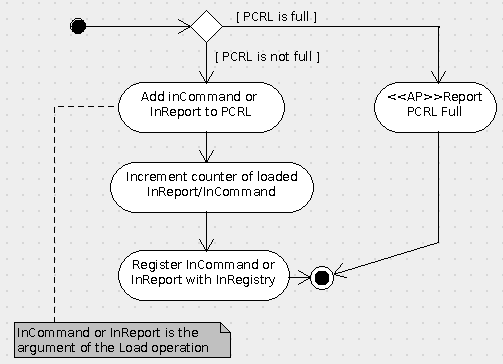
\includegraphics[scale=0.45,keepaspectratio=true]{InManagerLoad.png}
 \caption{The InManager Load Procedure}
 \label{fig:InManagerLoad}
\end{figure}

The InManager component is defined as an extension of the Base Component of section \ref{sec:BaseCmp}. It uses the \textit{Execution Procedure} of the Base Component to process the pending commands and reports. The InManager component processes the pending commands and reports by sending them an \texttt{Execute} command and a \texttt{Terminate} command (note that the \texttt{Terminate} command has no effect on an InReport).

After the \texttt{Terminate} command, the state of the InCommand or InReport is reported to the InRegistry using the latter \texttt{Update} operation (see section \ref{sec:InRegistry}). InCommands which have terminated execution are removed from the PCRL and are returned to the InFactory. InReports are returned to the InFactory after their first execution. The \textit{Execution Procedure} of the InManager is shown in figure \ref{fig:InManagerExecution}.

Normally, the InManager is embedded within a Real Time Container (see \cite{ref:fwprofile}) which is responsible for executing it. Thus, an application that is required to process commands and reports at different levels of priority should use several InManagers (one for each level of priority) and should allocate them to Real Time Containers with a matching priority.

\begin{figure}[H]
 \centering
 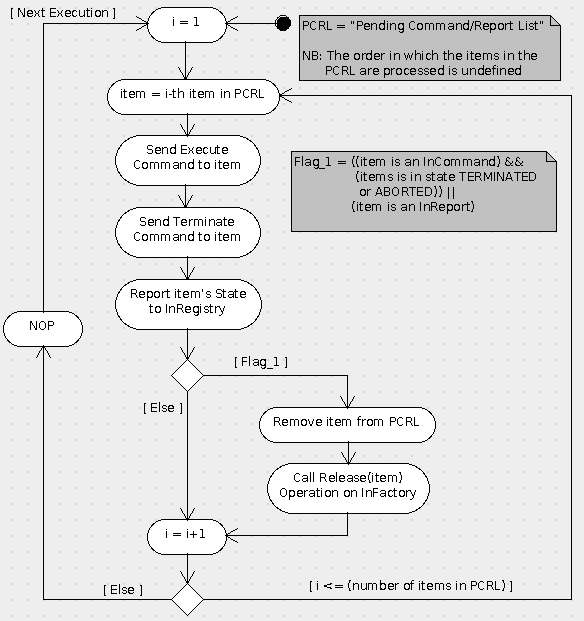
\includegraphics[scale=0.35,keepaspectratio=true]{InManagerExecution.png}
 \caption{The InManager Execution Procedure}
 \label{fig:InManagerExecution}
\end{figure}

